\documentclass[journal]{vgtc}                % final (journal style)
%\documentclass[review,journal]{vgtc}         % review (journal style)
%\documentclass[widereview]{vgtc}             % wide-spaced review
%\documentclass[preprint,journal]{vgtc}       % preprint (journal style)
%\documentclass[electronic,journal]{vgtc}     % electronic version, journal

%% Uncomment one of the lines above depending on where your paper is
%% in the conference process. ``review'' and ``widereview'' are for review
%% submission, ``preprint'' is for pre-publication, and the final version
%% doesn't use a specific qualifier. Further, ``electronic'' includes
%% hyperreferences for more convenient online viewing.

%% Please use one of the ``review'' options in combination with the
%% assigned online id (see below) ONLY if your paper uses a double blind
%% review process. Some conferences, like IEEE Vis and InfoVis, have NOT
%% in the past.

%% Please note that the use of figures other than the optional teaser is not permitted on the first page
%% of the journal version.  Figures should begin on the second page and be
%% in CMYK or Grey scale format, otherwise, colour shifting may occur
%% during the printing process.  Papers submitted with figures other than the optional teaser on the
%% first page will be refused.

%% These three lines bring in essential packages: ``mathptmx'' for Type 1
%% typefaces, ``graphicx'' for inclusion of EPS figures. and ``times''
%% for proper handling of the times font family.

\usepackage{enumerate}

\usepackage{mathptmx}
\usepackage{graphicx}
\usepackage{times}

%% We encourage the use of mathptmx for consistent usage of times font
%% throughout the proceedings. However, if you encounter conflicts
%% with other math-related packages, you may want to disable it.

%% This turns references into clickable hyperlinks.
\usepackage[bookmarks,backref=true,linkcolor=black]{hyperref} %,colorlinks
\hypersetup{
  pdfauthor = {},
  pdftitle = {},
  pdfsubject = {},
  pdfkeywords = {},
  colorlinks=true,
  linkcolor= black,
  citecolor= black,
  pageanchor=true,
  urlcolor = black,
  plainpages = false,
  linktocpage
}

%% If you are submitting a paper to a conference for review with a double
%% blind reviewing process, please replace the value ``0'' below with your
%% OnlineID. Otherwise, you may safely leave it at ``0''.
\onlineid{0}

%% declare the category of your paper, only shown in review mode
\vgtccategory{Research}

%% allow for this line if you want the electronic option to work properly
\vgtcinsertpkg

%% In preprint mode you may define your own headline.
%\preprinttext{To appear in an IEEE VGTC sponsored conference.}

%% Paper title.

\title{Hierarchical color palettes}

%% This is how authors are specified in the journal style

%% indicate IEEE Member or Student Member in form indicated below
\author{Martijn Tennekes and Edwin de Jonge}


\authorfooter{
%% insert punctuation at end of each item
\item
Martijn Tennekes, Statistics Netherlands. E-mail: m.tennekes@cbs.nl.
\item
Edwin de Jonge, Statistics Netherlands. E-mail: e.dejonge@cbs.nl.
}

%other entries to be set up for journal
\shortauthortitle{Biv \MakeLowercase{\textit{et al.}}: Hierarchical color palettes}
%\shortauthortitle{Firstauthor \MakeLowercase{\textit{et al.}}: Paper Title}

%% Abstract section.
\abstract{Color is an important means to display categorical data in statistical graphics. Categories are often hierarchically structured in a classification tree, but most color palettes do not take this hierarchy into account. We present a method to map tree structures to colors from the Hue-Chroma-Luminance (HCL) color model. The HCL color space is known for its well balanced perceptual properties. Our study suggest that hierarchical qualitative color palettes are very useful: not only for improving standard hierarchical visualizations such as trees and treemaps, but also for showing tree structure in non-hierarchical visualizations.
} % end of abstract

%% Keywords that describe your work. Will show as 'Index Terms' in journal
%% please capitalize first letter and insert punctuation after last keyword
\keywords{Color palettes, statistical graphics, hierarchical data.}

%% ACM Computing Classification System (CCS). 
%% See <http://www.acm.org/class/1998/> for details.
%% The ``\CCScat'' command takes four arguments.

\CCScatlist{ 
 \CCScat{H.5.2}{ Information Interfaces and Presentation}%
{User Interfaces}{User-centered design}
}


%% Uncomment below to include a teaser figure.
  \teaser{
  \centering
  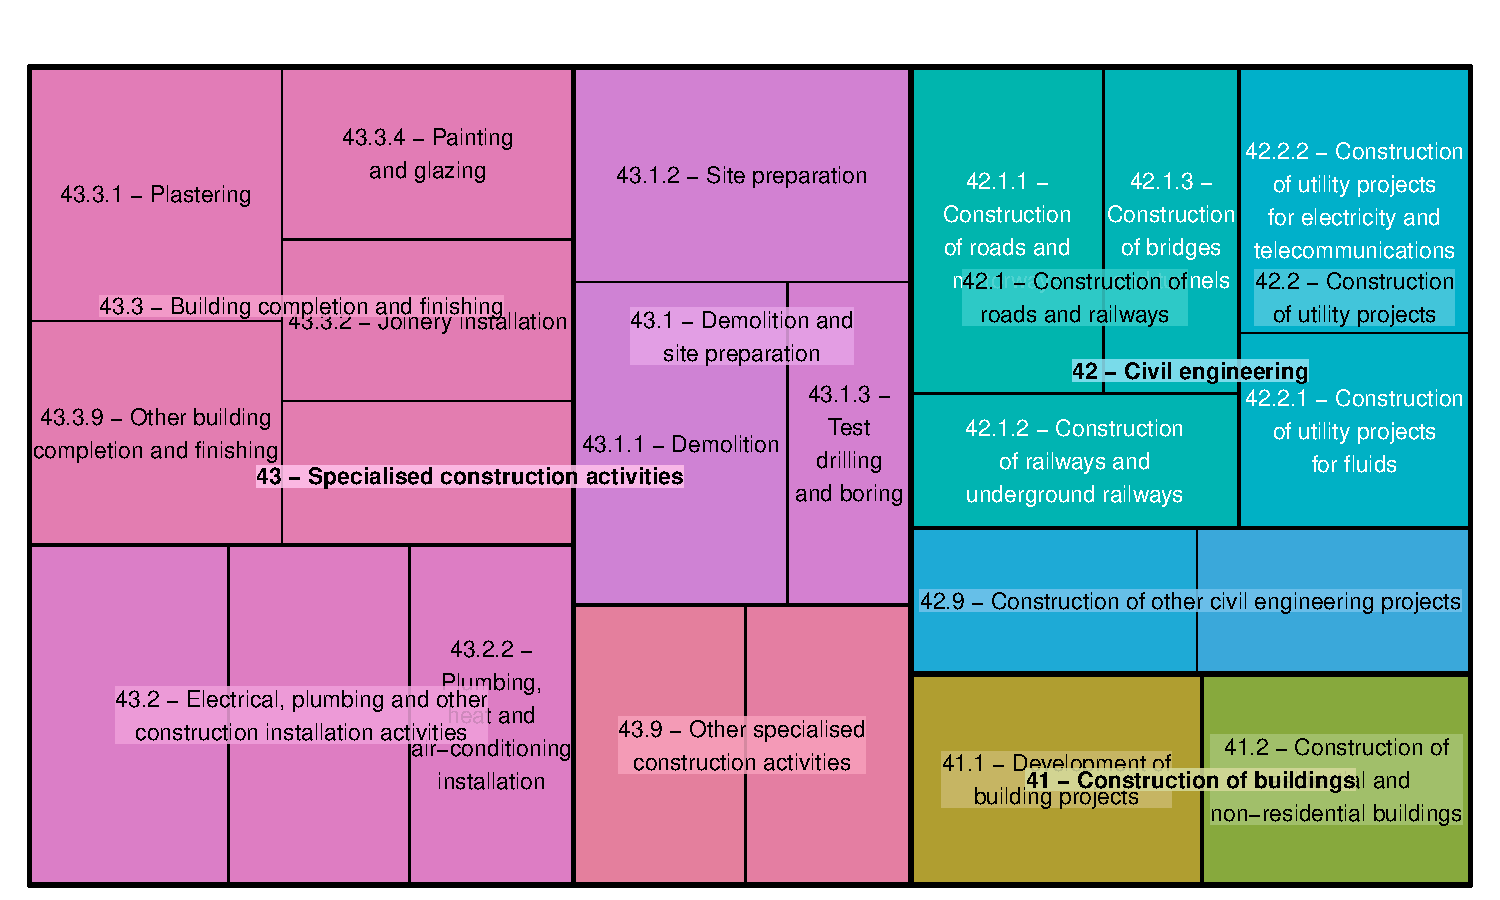
\includegraphics[width=16cm]{treemap_F.pdf}
  \caption{Treemap with hierarchical colors.}
  }

%% Uncomment below to disable the manuscript note
%\renewcommand{\manuscriptnotetxt}{}

%% Copyright space is enabled by default as required by guidelines.
%% It is disabled by the 'review' option or via the following command:
% \nocopyrightspace

%%%%%%%%%%%%%%%%%%%%%%%%%%%%%%%%%%%%%%%%%%%%%%%%%%%%%%%%%%%%%%%%
%%%%%%%%%%%%%%%%%%%%%% START OF THE PAPER %%%%%%%%%%%%%%%%%%%%%%
%%%%%%%%%%%%%%%%%%%%%%%%%%%%%%%%%%%%%%%%%%%%%%%%%%%%%%%%%%%%%%%%%


\graphicspath{{../plots/}}


\begin{document}

%% The ``\maketitle'' command must be the first command after the
%% ``\begin{document}'' command. It prepares and prints the title block.

%% the only exception to this rule is the \firstsection command
\firstsection{Introduction}

\maketitle

Hierarchical data are of crucial importance in official statistics. Most official data are published using hierarchically structured categories, for instance geographic regions or economic activities. Several data visualization methods are useful to explore and analyze hierarchical statistical data, for instance treemaps
\cite{shneiderman1992,tennekes2011b}. Color palettes reflecting the  hierarchical structure would be very useful in supporting visual analysis.

Assigning colors to categories is far from trivial. On the one hand, qualitative colors should be distinct, but on the other hand they should not suggest non-existent order or proximity and introduce perceptual bias. The selection of color palettes for categorical data first depends on the type of data. For nominal data, such as gender or nationality, qualitative color palettes are used, while for ordinal data, such as level of urbanization, sequential or diverging palettes are used \cite{brewer03, zeileis2009}. However, for hierarchical categories there are no specific guidelines for selecting color palettes, to the best of our knowledge.

Although many tree visualizations are proposed in literature \cite{schulz2011}, most of them use color to a small extent. A visualization technique that uses color as a major attribute is the InterRing \cite{yang2002}, a navigation tool with a radial layout. The leaf nodes are assigned to a different hue values. The color of a parent node is derived from averaging the colors of its children, where larger branches have more weight. An implicit effect is that colors of higher hierarchical levels are less saturated, except for one-child-per-parent branches.


\section{Method}
Our method maps a tree structure on colors in HCL space, such that it reflects the hierarchical properties of the tree. The Hue-Chroma-Luminance (HCL) space, which is a transformation of the CIELUV color space, is designed with the aim to control human color perception~\cite{ihaka2003}.
Colors with different hue values are perceptually uniform in colorfulness and brightness, which does not hold for the popular Hue-Saturation-Value (HSV) color space~\cite{zeileis2009}. 
%The hue $H$ takes values from 0 to 360, and the chroma $C$ and luminance $L$ take values from 0 to 100.


We use $H$, with range [0, 360], for the tree structure, where the hue of each child node resembles the hue of its parent. $C$ and $L$, both with range [0, 100], are used to discriminate the different hierarchical levels.

In this paper we illustrate our method with the European classification system of economic activity NACE. Figure~\ref{fig:sbiF} show a small part of the NACE: section F (Construction). Figure~\ref{fig:sbiF} is a typical tree visualization using a radial layout, but is improved by using nodes with colors from our hierarchical color palette. 

\begin{figure}[htb]
  \vspace{-3ex}
  \centering
  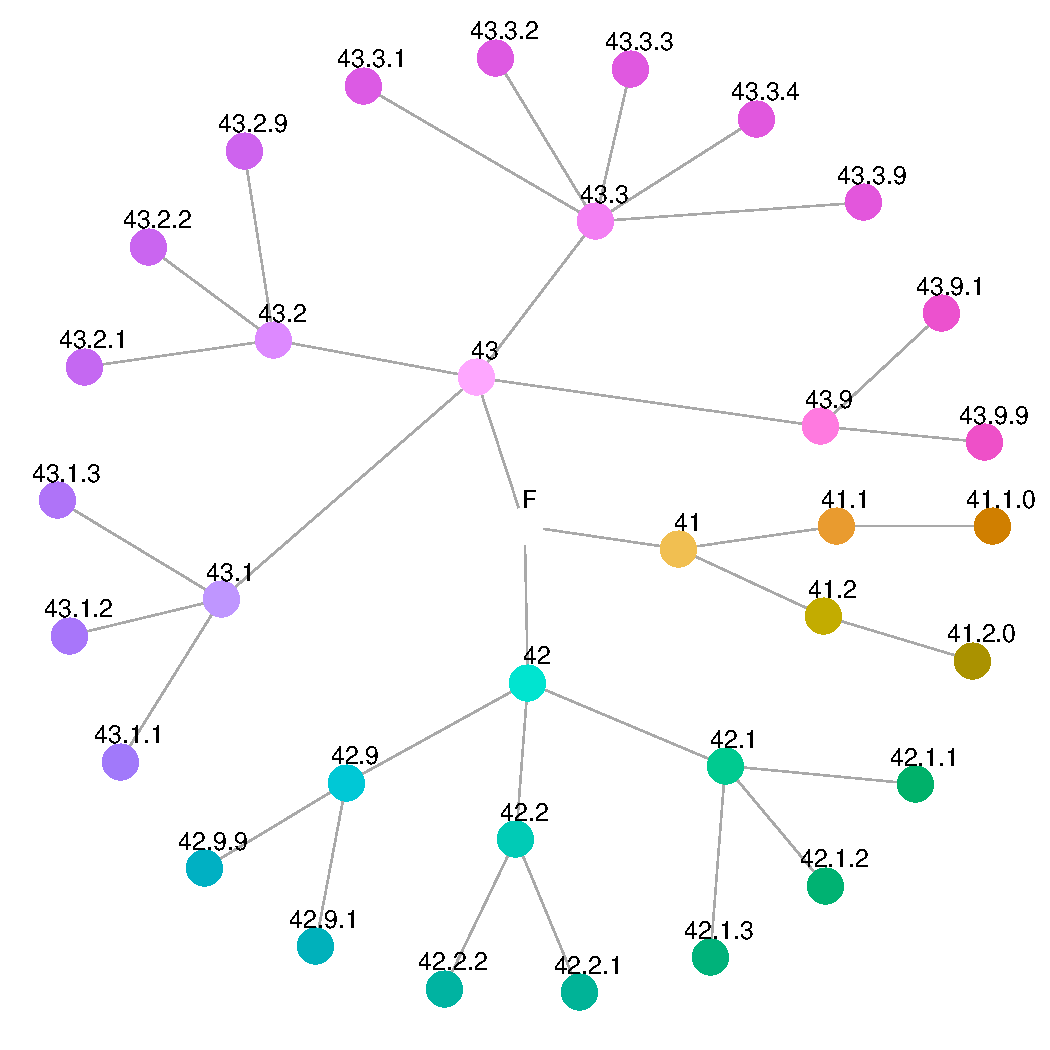
\includegraphics[width=3.2in]{sbi_F.pdf}
  \vspace{-5ex}
  \caption{Tree structure of economic sector F of NACE.}\label{fig:sbiF}
  \vspace{-2ex}
\end{figure}

For selecting hue values we use the following recursive algorithm. It will assign to each node $v$ of a tree structure a hue value $h$ and a hue value range $r$.
We start with the root node, which has by default hue range $[0, 360]$:

\smallskip{\bf AssignHue($v$, $r$)}
\vspace{-1mm}\begin{enumerate} \itemsep1pt \parskip0pt 
\parsep0pt
\item assign the middle hue value in $r$ to $h$ \footnote{In most cases the root node itself will not be drawn.}
\item $N$ is number of child nodes of $v$, if $N>0$ :
\begin{enumerate}[i] \itemsep1pt \parskip0pt 
\parsep0pt
\item divide $r$ in $N$ equal parts $r_i$;
\item permute the $r_i$'s and assign them to the child nodes
\item reduce each $r_i$ by keeping the middle fraction $f$;
\item for each child node $v_i$ DO AssignHue($v_i$,$r_i$)
\end{enumerate}
\end{enumerate}

\begin{figure}[htb]
  \centering
  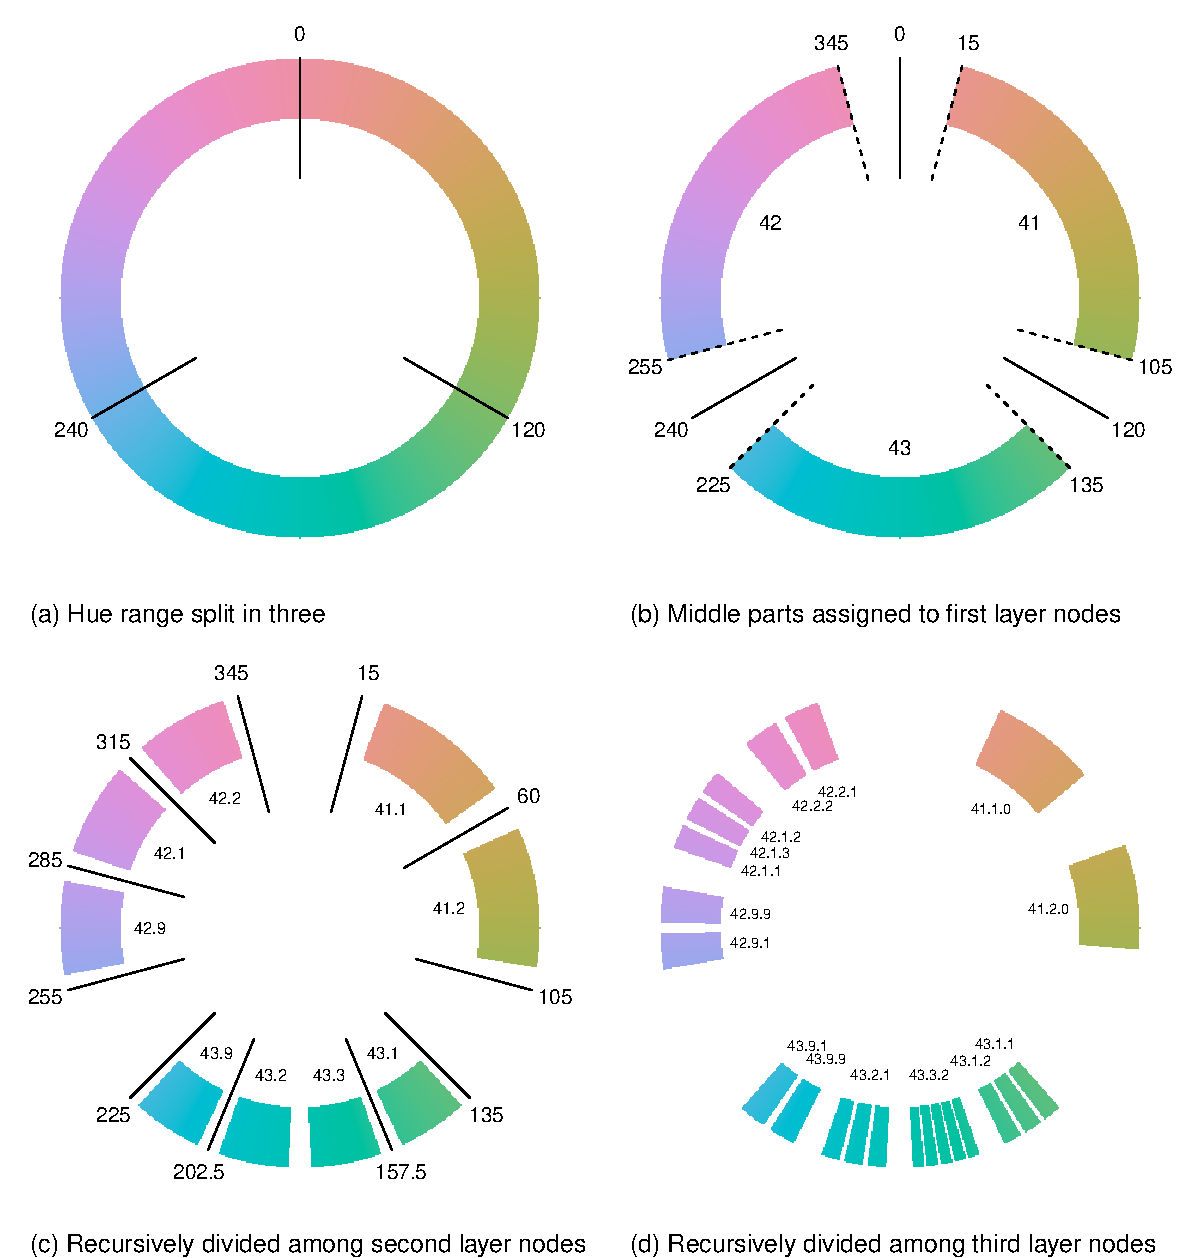
\includegraphics[width=3.5in]{hcl_method.pdf}
  \vspace{-5ex}
  \caption{Assignment of hue values.}\label{fig:wheel}
  \vspace{-4ex}
\end{figure}

This division of the hue range is illustrated in Figure~\ref{fig:wheel}: in (a) the full hue range (for a constant $C=60$ and $L=80$)  is divided and permuted among the three children of the root, in (b) the middle fractions are kept, in (c) and (d) these steps are recursively taken for the deepest two hierarchical layers.

Ad 2ii) In most hierarchical structures, there is no order between siblings. When the nodes in such structure are plotted in a linear or radial layout, the colors of the siblings should not introduce a perceptual order. Therefore, the assigned hue ranges are permuted among the siblings. The used permutation order is based on the five-elements-permutation $[1, 3, 5, 2, 4]$. Furthermore, the permutation within even numbered branches is reversed to differentiate between branches. Note the labeling of the color wheel that shows that the assignment of colors is permuted.

Ad 2iii) The fraction is needed to introduce a `hue gap' between nodes with a different parent. The fraction $f$ is by default set to $0.75$. This choice is a trade-off between discriminating different main branches and discriminating different leaf nodes. 

In order to show depth, we let $C$ and $L$ values only depend on the depth of the corresponding nodes in the tree structure. We let the $L$ decrease linearly with depth and $C$ increase: having more intense colors helps in discriminating leaf nodes.

\begin{figure}[htb]
  \vspace{-4ex}
  \centering
  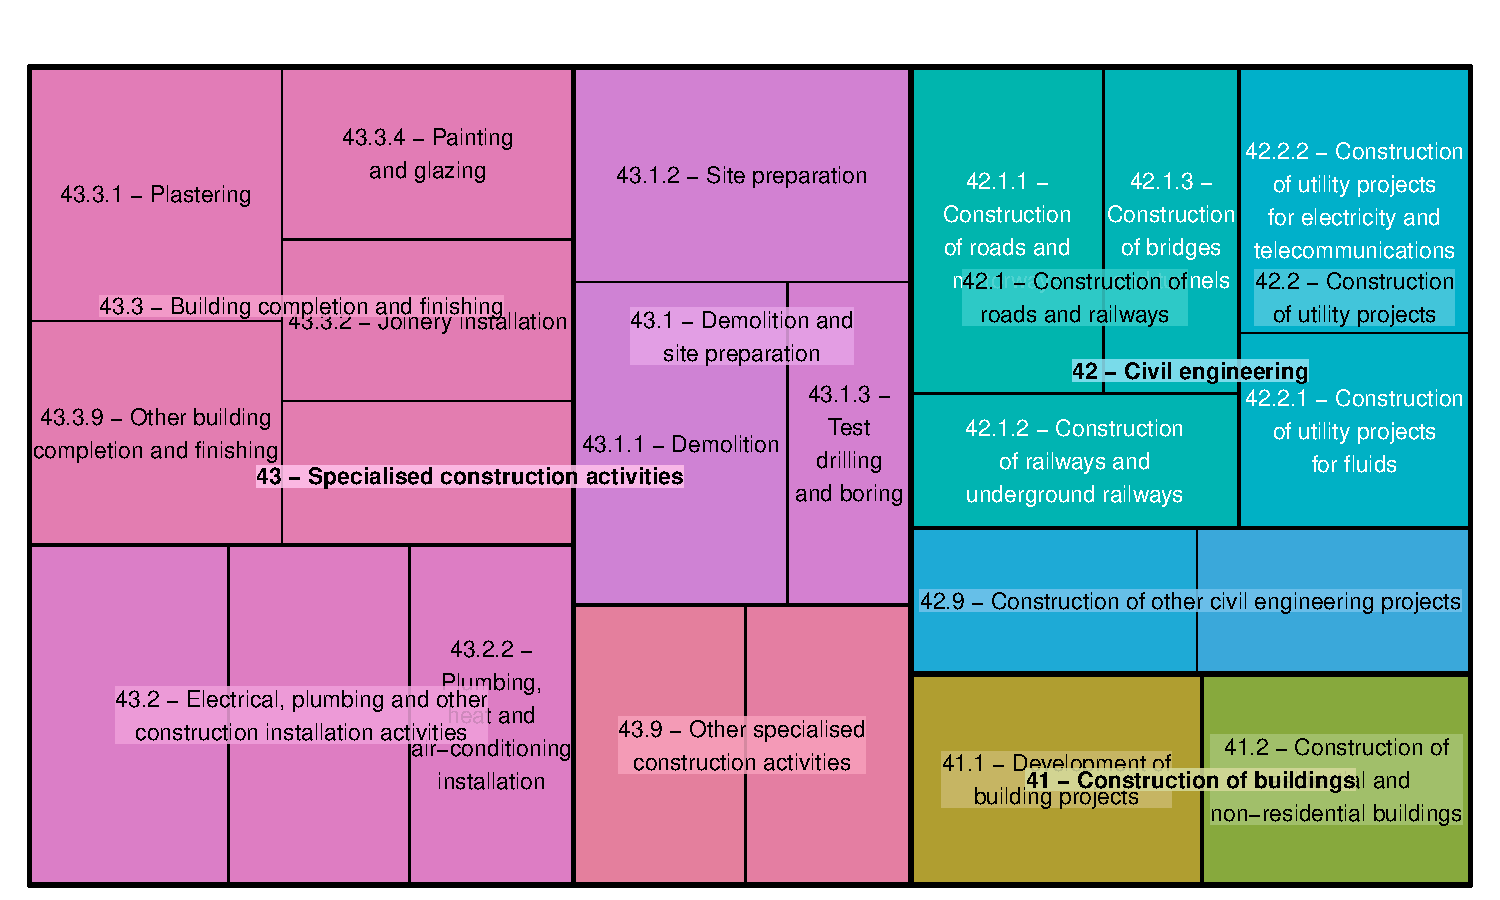
\includegraphics[width=3.5in]{treemap_F.pdf}
  \vspace{-4ex}
  \caption{Treemap with hierarchical colors}\label{fig:treemapF}
  \vspace{-4ex}
\end{figure}



\begin{figure}[htb]
  \centering
  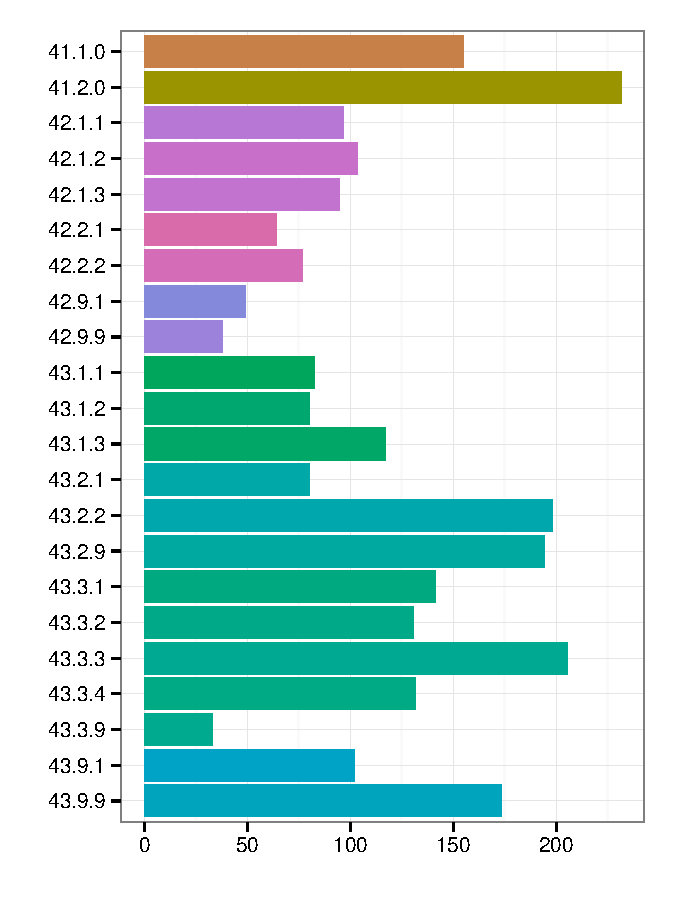
\includegraphics[width=1.235in]{bar_chart.pdf}
  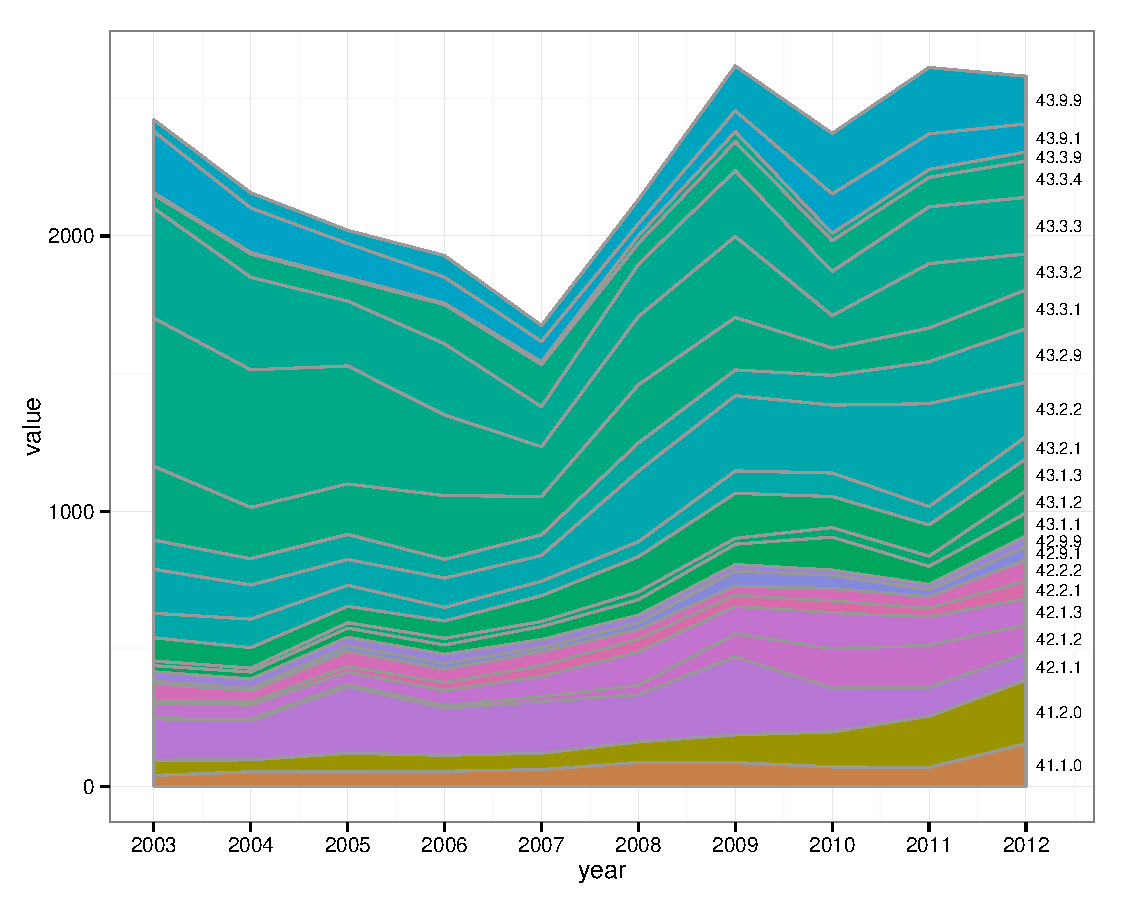
\includegraphics[width=2.065in]{stackedarea_chart.pdf}
  \vspace{-5ex}
  \caption{Bar chart and stacked area chart with hierarchical colors}\label{fig:charts}
  \vspace{-4ex}
\end{figure}

%\begin{figure}[htb]
%  \centering
%  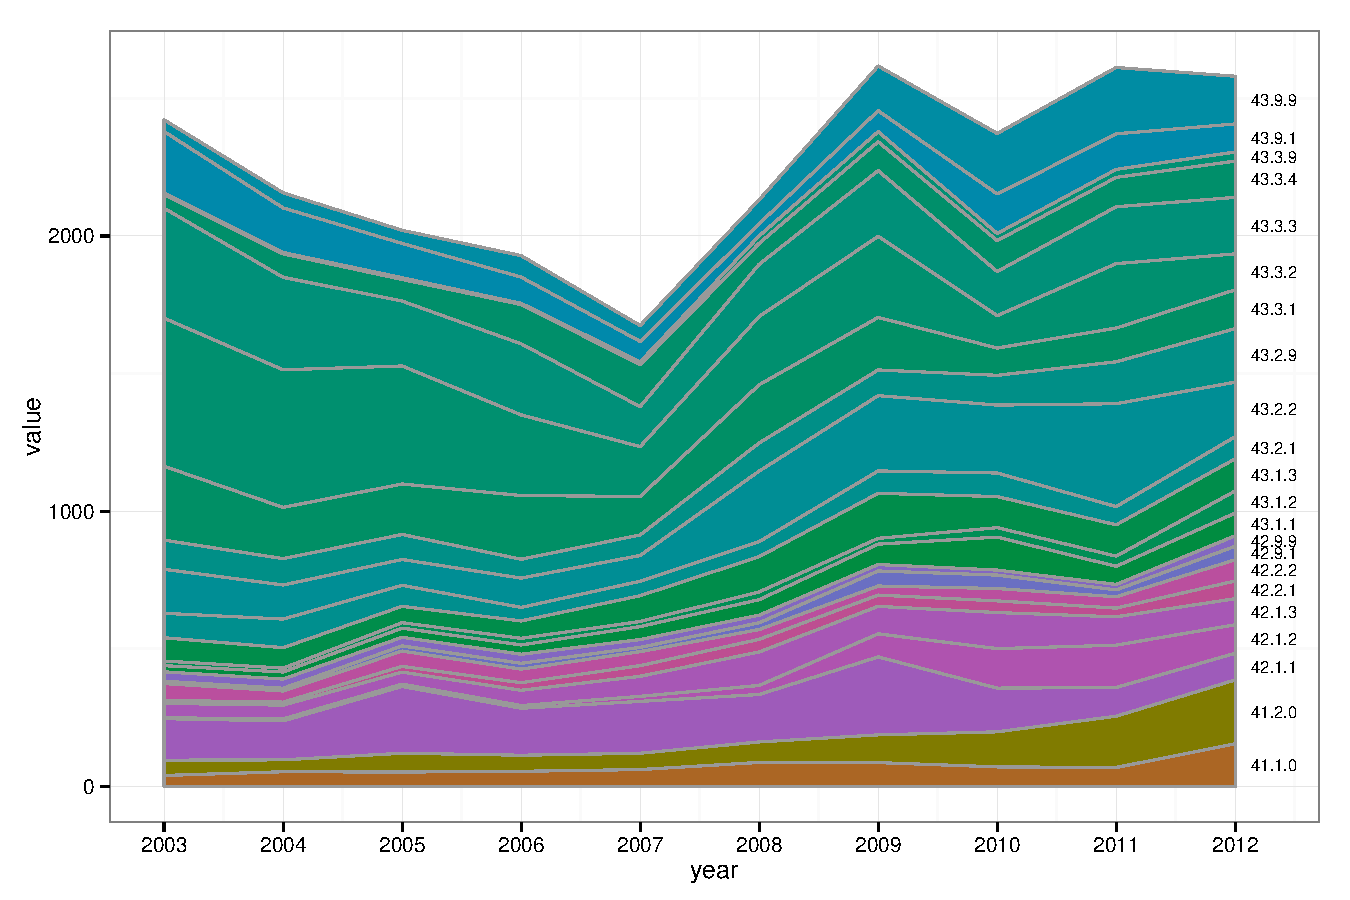
\includegraphics[width=0.25in]{stackedline_chart.pdf}
%  \caption{Stacked line chart with hierarchical colors}\label{fig:linechart}
%\end{figure}
%\begin{figure}[htb]
%  \centering
%  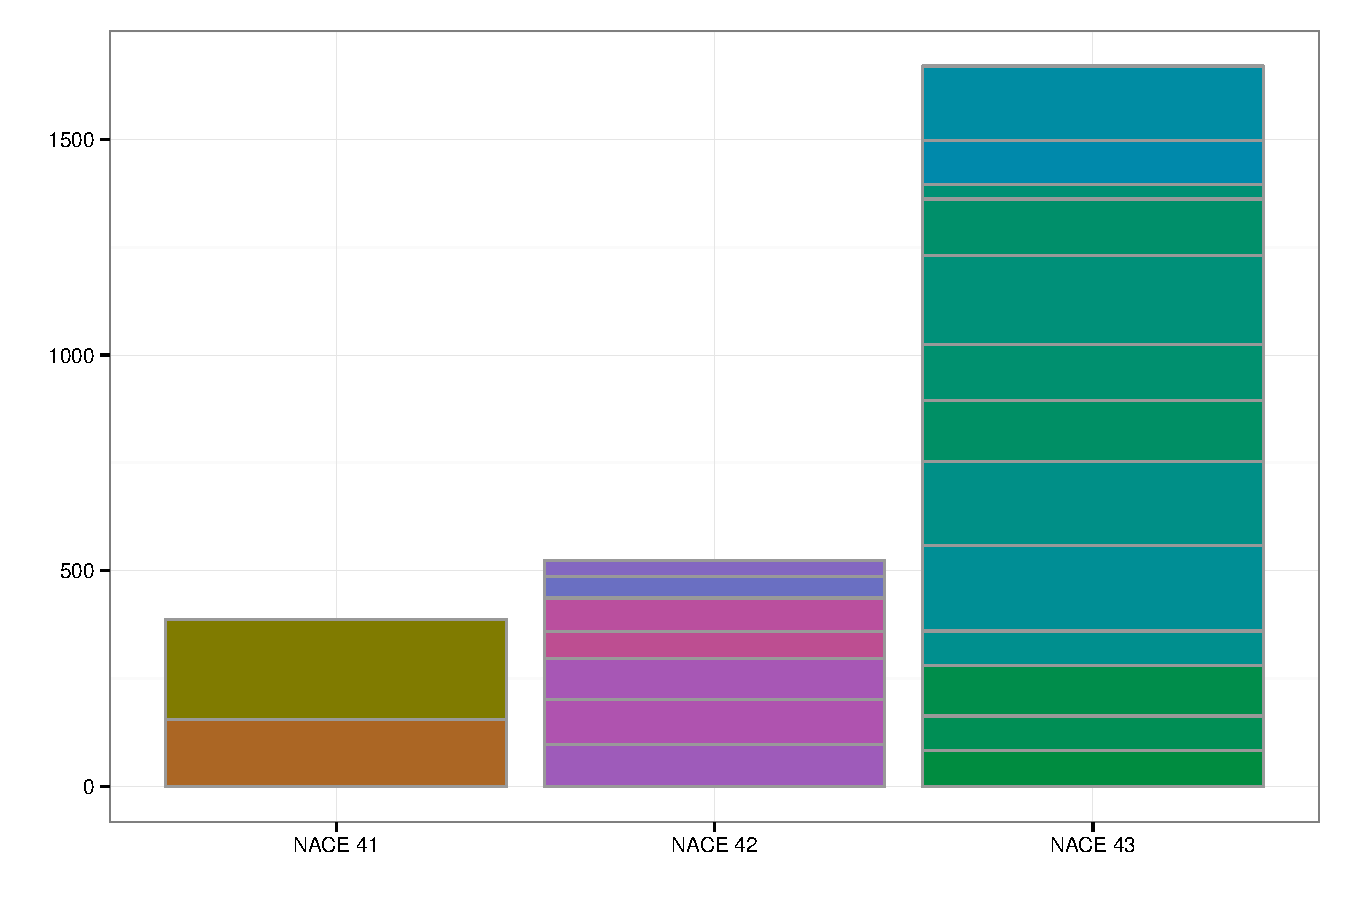
\includegraphics[width=1.75in]{stackedbar_chart.pdf}
%  \caption{Stacked bar chart with hierarchical colors}\label{fig:barchart}
%\end{figure}



\section{Application}
The hierarchical colors can be applied to enhance standard tree visualizations, as we saw in Figure~\ref{fig:sbiF}. Strictly speaking this is redundant color usage, but in our opinion it can improve many tree visualizations, because branches can be distinguished more easily. 

A second example of improvement is depicted in Figure~\ref{fig:treemapF}. It shows a treemap depicting (fictious) turnover values in Construction (NACE F). In official statistics, turnover is available for each business enterprise in a business register, and aggregated according to the NACE tree. The hierarchical color palette is used to differentiate between different aggregated groups, that makes it possible to compare turnover values at different hierarchical layers. Although the colors of higher NACE layers are only used for the text label backgrounds, they are also resembled by the colors of the lowest NACE layers. This treemap is created with the free and open source R package treemap \cite{treemap}.

Hierarchical colors can also improve visualizations without explicit tree structure. The colors hint at the underlying tree structure.
To illustrate this, a bar chart and a stacked area chart of fictive turnover data are depicted in Figure~\ref{fig:charts}. Such graphics could be useful when the hierarchical structure will not be the main focus in the conducted analyses. The bar chart can be used to compare turnover values of all leaf node sectors in Construction (NACE F), and the stacked area plot to analyse turnover values in time.

\section{Concluding remarks}
In our opinion, the proposed method to create hierarchical color palettes improves statistical visualizations, both hierarchically and non-hierarchically structured. The pre-condition that colors in the same hierarchical layer should be similar in terms of colorfulness and brightness it satisfied. This property is especially important in statistical visualizations, since they aim to visualize data as objectively as possible. The downside of the proposed method is that some leaf node colors will still be hard to distinguish.

We recommend a user study to evaluate the obtained hierarchical color palettes when applied in various statistical visualizations. The main aim of this user study would be to find out whether hierarchical palettes are useful in statistical analysis.


%% if specified like this the section will be committed in review mode
\acknowledgments{
The authors wish to thank their collegues at Statistics Netherlands who participated in the user survey.}

\bibliographystyle{abbrv}
%%use following if all content of bibtex file should be shown
%\nocite{*}
\bibliography{hcp}
\end{document}
